\documentclass[conference]{IEEEtran}
\IEEEoverridecommandlockouts
% The preceding line is only needed to identify funding in the first footnote. If that is unneeded, please comment it out.
\usepackage{cite}
\usepackage{amsmath,amssymb,amsfonts}
\usepackage{algorithmic}
\usepackage{graphicx}
\usepackage{textcomp}
\usepackage{xcolor}
\usepackage{comment}
\def\BibTeX{{\rm B\kern-.05em{\sc i\kern-.025em b}\kern-.08em
    T\kern-.1667em\lower.7ex\hbox{E}\kern-.125emX}}
\begin{document}

\title{SMDE Assignment}

\author{\IEEEauthorblockN{1\textsuperscript{st} Carles Matoses}
\IEEEauthorblockA{carles.matoses@estudiantat.upc.edu}
\and
\IEEEauthorblockN{2\textsuperscript{nd} Ignasi Granell}
\IEEEauthorblockA{ignasi.granell@estudiantat.upc.edu}
\and
\IEEEauthorblockN{3\textsuperscript{rd} Isabel Castañeda}
\IEEEauthorblockA{isabel.castaneda@estudiantat.upc.edu}
}

\maketitle

\section{Problem description}
% add the issues you detect. 
% In the Marathon, are enough resources for the runners? (WC, water sources, meals…), there are some unexpected queues, what about make the race on august?
We are provided with three marathon results, from a Kaggle dataset, on the years 2015, 2016 and 2017. The data is structured in a way that we have the runners' information, the time they took to get to interest points and the time they took to finish the race. Some of the most relevant variables we are provided are: the age, the gender and the city of origin. We believe this characteristics have a direct impact on the performance of the runners.

Reading the paper \cite{b8}, we concluded that, effectively, environmental conditions have a direct impact on the performance of runners. The paper states that the temperature has a positive impact (longer races) and high humidity and high wind speed have a negative impact on the performance of the runners (faster races).

% Some ideas about this (since i do not know what the proffessor wants):
% - The temperature analysis only takes into account a small range of 5◦C to 24.5◦C, maybe results would be different if we consider hotter enviorments.
% - The wind speed analysis does not seem to explain wind direction. Maybe its usually the same direction in this place
% 
\section{System description, introduction}
% Describe the system to be modeled (not the problem, not the data), other elements must be described on the subsequent sections of the document.
% Do we need to define what a system is? I don't think so
The system to be modelled is the ``Barcelona Marathon''. This marathon involves runners of different skill levels, ages, and genders, coming from various cities. The event is influenced by environmental factors such as humidity and temperature, all of which can impact runner performance. 

Runners rely on essential supplies, including water, food, and medical assistance, to complete the marathon safely. The course is structured as a linear system, where participants progress from one checkpoint to the next. Along the way, they encounter resupply points, which have limited capacities. If demand exceeds supply, queues may form, potentially delaying runners. Environmental conditions also play a significant role in the system, affecting both individual runner performance and the overall flow of the event.

Using this model we have determined that the best time to hold the race should be when temperature is low and humidity high, around autumn. We have also detected that poor allocation of supply stations can cause bunching up of runners and long queues, especially at the start of the race. More capacity should be allocated towards the start while still ensuring there are enough supplies throughout the race, as they become more necessary towards the end.

\section{Model specification}
% We will build a simulation model that represents a set of runners and how the climate conditions affect them.
% Clearly define the model entities, operations and processes that defines the behavior of the model. We must use here DEVS, Petri Nets or SDL, but since we are not going to use those formal languages, define a flow diagram to simplify the definition of the model. Since we are using GPSS you can use the GPSS icons of the language.

For this model, the entities and attributes are the following:

% TODO: 
% - carles: esto esta mal, lo tendremos que ajustar a nuestro modelo
% - carles: lo he arreglado un poco añadiendo nuevos atributos y eliminando otros.
\begin{itemize}
    \item \textbf{Runners}: The runners are the main entities in the system. They have attributes such as age, genre, and city of origin. They interact with the system by running the marathon.
    \item \textbf{Temperature}: The temperature is an environmental attribute that affects the performance of the runners.
    \item \textbf{Humidity}: The humidity is an environmental attribute that affects the performance of the runners.
    \item \textbf{Level}: The level of a runner is determined randomly following the proportions of the groups in the Boston Marathon dataset. It affects the base time it takes a runner to complete one section of the marathon. Lower level runners follow distributions with larger means and standard deviations.
    \item \textbf{Gender}: The gender of a runner is determined randomly based on their level following the distribution in the Boston Marathon dataset. It affects how environmental attributes affect their run time.
\end{itemize}

The operations of the model will be reduced to runners arriving at the end line. The processes of the model will be the following:
\begin{itemize}
    \item \textbf{Generate runners}: The simulation generates and initializes the runners's own attributes.
    \item \textbf{Start section}: The runner starts running.
    \item \textbf{Run}: The runner advances to the checkpoint.
    \item \textbf{Queue}: The runner enters the queue for resupplying.
    \item \textbf{Resupply}: The runner resupplies and leaves the queue.
    \item \textbf{Next section}: The runner moves back to "Start section" unless this is the last section.
    \item \textbf{End}: The runner finishes the race and the entity is terminated.
\end{itemize}

A diagram of the model is provided in figures \ref{fig:init_diagram}, \ref{fig:model_diagram}, \ref{fig:end_diagram} and \ref{fig:aux_diagram}. The full GPSS code is provided in the annex.

\begin{figure}[]
    \centerline{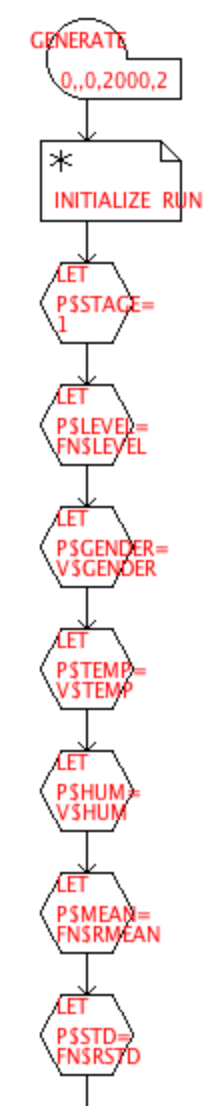
\includegraphics[width=0.2\linewidth]{figs/init_diag.png}}
    \caption{Generation and initialization of entities.}
    \label{fig:init_diagram}
\end{figure}

\begin{figure}[]
    \centerline{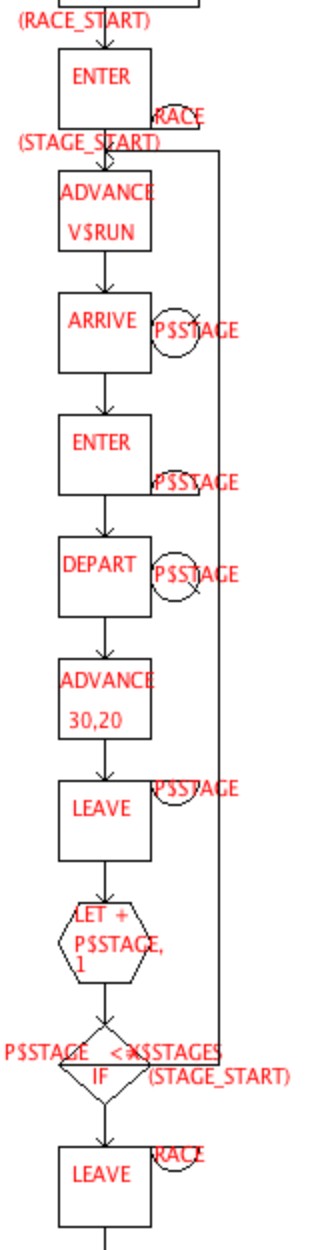
\includegraphics[width=0.2\linewidth]{figs/model_diag.png}}
    \caption{Main race flowchart.}
    \label{fig:model_diagram}
\end{figure}

\begin{figure}[]
    \centerline{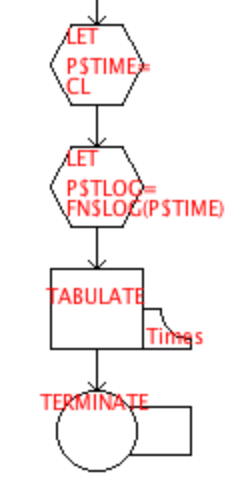
\includegraphics[width=0.2\linewidth]{figs/end_diag.png}}
    \caption{End of the race and data processing.}
    \label{fig:end_diagram}
\end{figure}

\begin{figure}[]
    \centerline{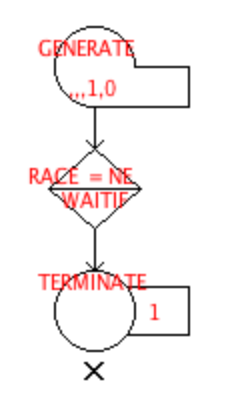
\includegraphics[width=0.2\linewidth]{figs/aux_diag.png}}
    \caption{Auxiliary process for ending the simulation.}
    \label{fig:aux_diagram}
\end{figure}


In this process, the model will use a normal distributed random variable to determine the time it takes a runner to finish. We created different time ranges to decide the level of a runner. The ``Elite'' runners tend to run 5 km in less than 18 minutes, the ``hobby'' runners take more than 18 minutes and less than 25 and ``new'' runners take more than 25 minutes.

The model purpose differs from the system purpose. We aim to predict the consequences of the environmental conditions on the performance of the runners. The model will help us understand how the humidity, heat, and other variables affects the performance of the runners. Additionally we want to measure the possible effects of bottlenecks due to supply constraints.


% I need to know the time required for an elite male runner to finish the race. and then the female elite runner.

\subsection{Systemic Structural, Systemic Data and Simplifying Hypotheses}

\begin{itemize}
    \item \textbf{SS\_01}: The runners will be split in three ``level'' groups based on the performance of the first 5 km. Different groups run at different speeds.
    \item \textbf{SS\_02}: Temperature and humidity will affect the speed of runners.
    \item \textbf{SS\_03}: After each sector there will be a resupply point and runners will queue for it.
    \item \textbf{SS\_04}: The race will have 10 sectors.
    \item \textbf{SH\_01}: Runners will keep a constant speed over each sector, the average speed over all sectors will be the same.
    \item \textbf{SH\_02}: Male and female runners will have the same based speed according to their level.
    \item \textbf{SH\_03}: Runners take an average of 30 seconds to resupply, following a uniform distribution of 20 seconds of half spread.
    \item \textbf{SD\_04}: All runners are affected by environmental effects in the same way according to their gender.
    \item \textbf{SD\_01}: The 3 level groups represent statistically different groups with different times and paces.
    \item \textbf{SD\_02}: The log of the total time is approximate enough to a normal distribution.
\end{itemize}

% TODO: maybe remove the 
\begin{table}[htbp]
\caption{Environmental Impact on Marathon Performance}
\begin{center}
\begin{tabular}{|c|c|c|}
\hline
\textbf{} & \textbf{MAN: mean, std. dev.} & \textbf{WOMAN: mean, std. dev.} \\
\hline
\textbf{Humidity} & & \\
\hline
low & 0, 0 & 0, 0 \\
\hline
medium & -1.73, 0.22 & -1.74, 0.28 \\
\hline
high & -2.11, 0.2 & -0.90, 0.34 \\
\hline
\textbf{Temperature} & & \\
\hline
low & 0, 0 & 0, 0 \\
\hline
medium & 1.19, 0.19 & 1.38, 0.23 \\
\hline
high & 7.73, 0.18 & 7.78, 0.38 \\
\hline
\textbf{Wind Speed} & & \\
\hline
low & 0, 0 & 0, 0 \\
\hline
medium & -3.18, 0.2 & -1.90, 0.32 \\
\hline
high & -4.92, 0.2 & -0.87, 0.3 \\
\hline
\end{tabular}
\label{tab:environmental_impact}
\end{center}
\end{table}

\begin{table}[htbp]
\caption{Gender Percentage in Runner Groups}
\begin{center}
\begin{tabular}{|c|c|c|c|}
\hline
\textbf{Group} & \textbf{Male (\%)} & \textbf{Female (\%)} & \textbf{Total (\%)} \\
\hline
Elite Runners & 93.61 & 6.39 & 0.82 \\
\hline
Hobby Runners & 70.30 & 29.70 & 49.23 \\
\hline
New Runners & 38.74 & 61.26 & 49.38 \\
\hline
\end{tabular}
\label{tab:gender_percentage}
\end{center}
\end{table}

\section{Coding}
\subsection{Data}
Temperature and precipitations are extracted from the years 1950 to 2019 from the meteorologic service of Barcelona. The wind speed and humidity are extracted from the same source but years 2007 to 2016.
Race times are extracted from the marathon results of 2015. We calculated the mean and standard deviation of each group: elite, hobby, and new runners. The results are shown in table \ref{tab:elite_hobby_new_mean_std_dev}.

\begin{table}[htbp]
\caption{Mean and Standard Deviation of Race Times for Runner Groups}
\begin{center}
\begin{tabular}{|c|c|c|}
\hline
\textbf{Group} & \textbf{Mean Time (min)} & \textbf{Standard Deviation (min)} \\
\hline
Elite Runners & 153.92 & 10.66 \\
\hline
Hobby Runners & 198.63 & 19.24 \\
\hline
New Runners & 255.00 & 35.26 \\
\hline
\end{tabular}
\label{tab:elite_hobby_new_mean_std_dev}
\end{center}
\end{table}

\begin{table}[htbp]
\caption{Monthly Temperature and Wind Data}
\begin{center}
\begin{tabular}{|c|c|c|c|}
\hline
\textbf{Month} & \textbf{Max Temp (°C)} & \textbf{Min Temp (°C)} & \textbf{Wind (km/h)} \\
\hline
Jan & 11.11 & 5.28 & 16.95 \\
\hline
Feb & 12.22 & 5.46 & 14.25 \\
\hline
Mar & 14.65 & 7.30 & 14.80 \\
\hline
Apr & 16.89 & 8.95 & 12.90 \\
\hline
May & 20.53 & 12.32 & 14.00 \\
\hline
Jun & 24.60 & 16.12 & 10.65 \\
\hline
Jul & 27.84 & 19.00 & 17.65 \\
\hline
Aug & 27.71 & 19.08 & 12.75 \\
\hline
Sep & 24.42 & 16.67 & 12.10 \\
\hline
Oct & 19.99 & 13.23 & 15.85 \\
\hline
Nov & 14.74 & 8.83 & 15.15 \\
\hline
Dec & 11.75 & 6.22 & 16.35 \\
\hline
Avg & 18.00 & 11.00 & 14.00 \\
\hline
\end{tabular}
\label{tab:monthly_temp_wind}
\end{center}
\end{table}

\begin{table}[htbp]
\caption{Monthly Precipitation and Humidity Data}
\begin{center}
\begin{tabular}{|c|c|c|}
\hline
\textbf{Month} & \textbf{Precipitation (mm)} & \textbf{Humidity (\%)} \\
\hline
Jan & 42.74 & 68 \\
\hline
Feb & 36.53 & 65 \\
\hline
Mar & 51.46 & 64 \\
\hline
Apr & 54.91 & 67 \\
\hline
May & 58.24 & 65 \\
\hline
Jun & 37.25 & 60 \\
\hline
Jul & 28.75 & 63 \\
\hline
Aug & 43.68 & 65 \\
\hline
Sep & 73.14 & 68 \\
\hline
Oct & 88.29 & 72 \\
\hline
Nov & 62.91 & 69 \\
\hline
Dec & 47.32 & 67 \\
\hline
Avg & 55.00 & 66 \\
\hline
\end{tabular}
\label{tab:monthly_precip_humidity}
\end{center}
\end{table}
\section{Definition of the experimental framework}
\begin{enumerate}
    \item \textbf{Design of the DOE}
    
    To evaluate the effects of key factors on marathon performance, we implemented a basic Design of Experiments (DOE). The factors considered in this study are:
    \begin{itemize}
        \item \textbf{Temperature}: Low and high represent the effects of low temperature and high temperature as identified in the preliminary marathon study \cite{b8}. Medium temperature is also modelled but not tested.
        \item \textbf{Humidity}: Represented similarly as the effects of low and high humidity in the same study. Likewise medium humidity is not tested.
        \item \textbf{Supplies}: Low supplies represents the capacity to supply 200 people at once in any given supply point, high represents the capacity to supply 500 people at once.
    \end{itemize}

    Due to limitations in the version of GPSS we run only $1/10$th of the runners, 2000 in total, and also divide the supply availability by 10, taking the final values of 20 and 50.

    The primary goal of the DOE is to identify the optimal combination of these factors that minimises the average time it takes for runners to complete the race. In this context, “best” is defined as achieving the lowest average time while maintaining manageable resource usage. Additionally, we use analyse the queues formed during the runtime of the simulation to identify bottlenecks related to resource availability and how to best allocate them.
    
    The implementation uses functions to dynamically assign values for these factors to runners during the simulation. Each runner’s performance is calculated using the following formula:

    % I don't know how to put it smaller
    \[
        Run Time = \frac{e^t+Temp+Humidity}{Stages}
    \]

    Where $t$ is a random value following a normal distribution with the values identified from preliminary data analysis. This ensures that the impact of temperature, humidity, and supplies is directly incorporated into the simulation of each runner's race.

    \item \textbf{Execution of the Replications}
    
    The DOE is executed by:
    \begin{itemize}
        \item \textbf{Generating runners dynamically}: Runners are created and their properties are initialized following distributions from the Boston Marathon dataset.
        \item \textbf{Simulating the race}: The simulation progresses through 10 stages, with each runner advancing at a calculated pace based on the environmental factors and their personal attributes.
        \item \textbf{Replicating the experiment}: For each configuration of factors, multiple runners are simulated to provide robust results. Since this isn't a continuous system and has a defined start and end each replica of the experiment restarts the entire simulation. Each combination of high and low values is performed 16 times.
    \end{itemize}

    \item \textbf{Detection and Analysis of Interactions}
    The simulation setup inherently supports the evaluation of both main effects (e.g., how TEMP alone impacts performance) and interactions (e.g., how TEMP and HUM together influence results). The effects and interactions are computed using the Yates algorithm which can be found in the Annex.
    \item \textbf{Summary of Findings}
    Through running multiple replications of the simulation with different setups we identified that the main factor on the mean time to complete the race is the bottlenecks created by poor supply availability. As for climate effects the main factor is temperature, which should be minimized.
    % EXPAND
\end{enumerate}
\section{Model validation}
Validating the model is an essential step to ensure that it realistically represents the marathon and produces meaningful results. To achieve this, we applied several validation techniques as suggested in the literature \cite{math}. Each technique focuses on a specific aspect of the model’s accuracy and reliability.
% I defined 5 validations but we can decide which ones to do
% I commented these methods as we don't do them all

\begin{comment}
\begin{enumerate}
    \item \textbf{Conceptual Validation}
    \begin{itemize}
        \item \textbf{Objective}: To confirm that the model’s structure and assumptions are consistent with real-world behaviour.
        \item \textbf{Approach}: Reviewing the model’s assumptions, such as the simplification that runners maintain a constant speed within each stage, against insights from previous studies on marathon performance. Additionally, the logic and processes implemented in the simulation is compared with known dynamics of marathon events to ensure consistency.
    \end{itemize}
    \item \textbf{Data Validation}
        \begin{itemize}
        \item \textbf{Objective}: To verify that the input data is accurate and suitable for the simulation.
        \item \textbf{Approach}: Historical weather data from Observatori Fabra is cross-checked with official sources to ensure its reliability. Runners’ attributes, such as performance levels and physiological factors, are validated against publicly available datasets (e.g., Kaggle marathon data). Our assumptions about data are tested and confirmed against our input data.
    \end{itemize}
    \item \textbf{Dynamic Validation}
        \begin{itemize}
        \item \textbf{Objective}: To ensure the model’s behaviour aligns with expectations during the simulation.
        \item \textbf{Approach}: Step-by-step white-box checks of simulation outputs is conducted to verify that changes in inputs (e.g., temperature or humidity) produce logical trends, such as higher temperatures leading to longer completion times. A black box test is performed to verify the output is correct.
    \end{itemize}
    \item \textbf{Predictive Validation}
        \begin{itemize}
        \item \textbf{Objective}: To evaluate the model’s ability to replicate real-world results.
        \item \textbf{Approach}: Outputs from the simulation are compared to actual data from the Barcelona Marathon and other similar events, focusing on key metrics such as average completion times under comparable weather conditions.
    \end{itemize}
    \item \textbf{Statistical Validation}
        \begin{itemize}
        \item \textbf{Objective}: To ensure the results of the simulation are statistically robust and reliable.
        \item \textbf{Approach}: Statistical tests, including ANOVA, are used to evaluate whether differences in race times across various conditions are statistically significant. Tests for normality and variance homogeneity are applied to validate the assumptions required for further analysis.
    \end{itemize}

\end{enumerate}
\end{comment}

\subsection{Implemented Validation Methods}
\begin{enumerate}
    \item \textbf{Data Validation}
    First we validate our group categorization of runners's levels based on their time to reach 5km. Since we use the log of time for the simulaiton and analysis as it better approximates a normal distribution we run an ANOVA test on the equation $ln(time) ~ Level$. We checked the assumptions for the ANOVA test and found that while the normality of distribution is a bit off, the rest of the assumptions hold. The results of the ANOVA in table \ref{tab:anova_validation} show that there is a difference between at least one mean. A further Tukey HSD test reveals that all 3 means are different from each other, so our assumption that the 3 levels correspond to significantly different performance is validated.

    The second hypothesis to validate is that the log of time is close enough to a normal distribution. The results of the shapiro-wilk test and the  figures \ref{fig:elite_hobby_new_standar_deviation} and \ref{fig:new_qq} show that only elite runners follow a normal distribution, but while the other groups have some deviations, particularly at the extremes, the bulk of the dataset follows a roughly normal shape.

    \begin{figure}[htbp]
        \centerline{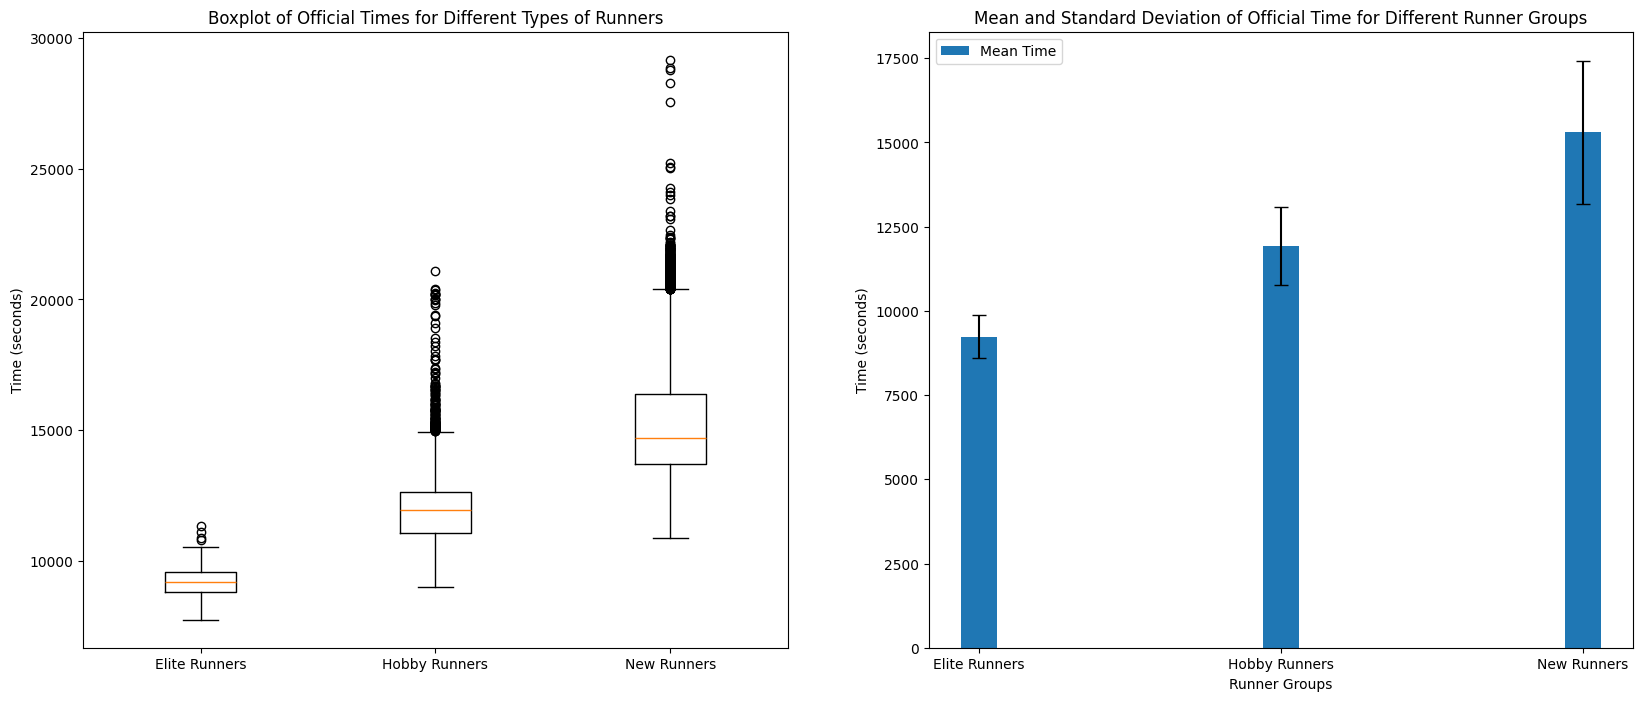
\includegraphics[width=\linewidth]{figs/elite_hobby_new_standar_deviation.png}}
        \caption{Standard deviation of race times for elite, hobby, and new runners.}
        \label{fig:elite_hobby_new_standar_deviation}
    \end{figure}
    
    \begin{figure}[htbp]
        \centerline{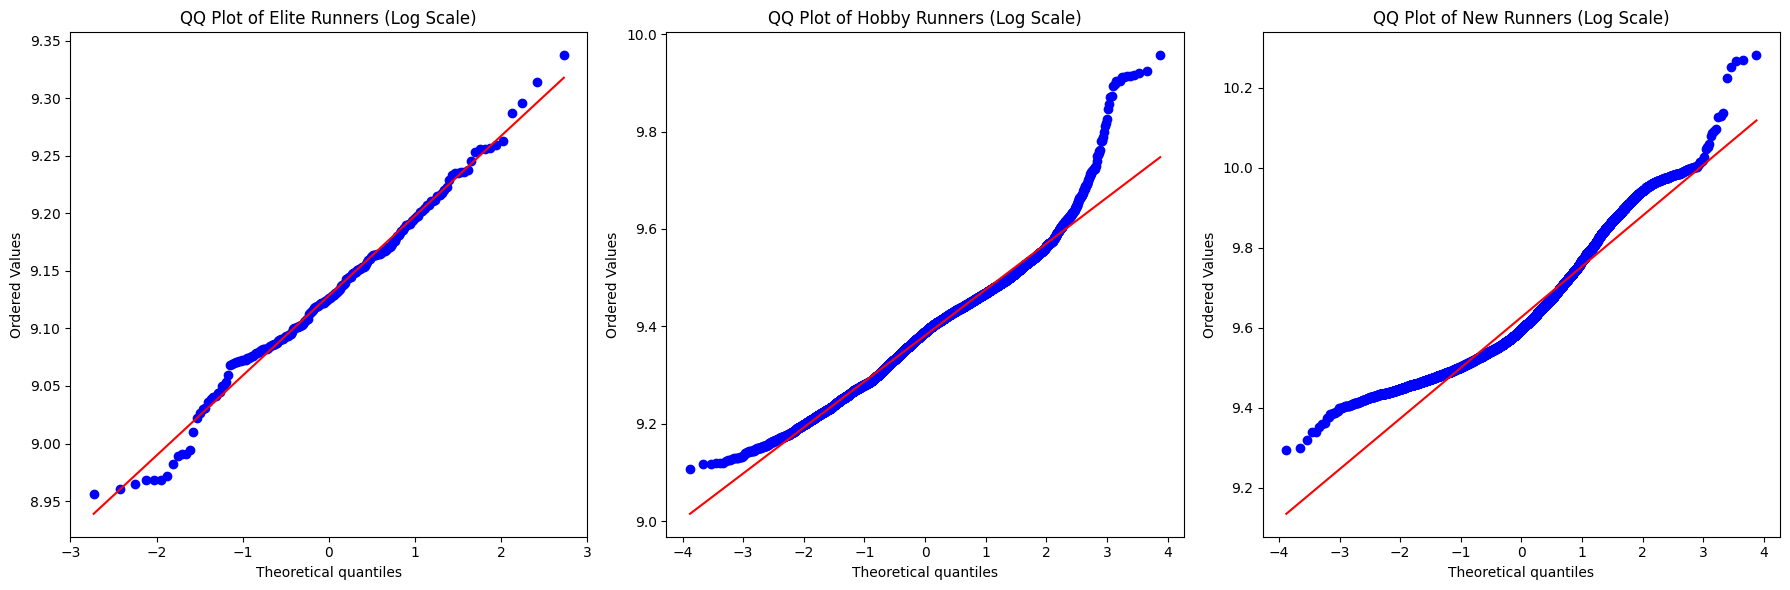
\includegraphics[width=\linewidth]{figs/elite_hobby_new_qq.png}}
        \caption{Q-Q plot for new runners.}
        \label{fig:new_qq}
    \end{figure}

    \begin{table}[htbp]
        \caption{ANOVA Table for runner groups}
        \begin{center}
        \begin{tabular}{|c|c|c|c|c|c|}
        \hline
            & \textbf{Df} & \textbf{Sum Sq} & \textbf{Mean Sq} & \textbf{F value} & \textbf{p value}\\
        \hline
        \textbf{Level} & 2&426.0&212.99&16387&\textless2e-16\\
        \hline
        \textbf{Residuals} & 26442&343.7&0.01&&\\
        \hline
        \end{tabular}
        \label{tab:anova_validation}
        \end{center}
        \end{table}

    \item \textbf{Dynamic Validation}
    During the programming of the simulation we performed dynamic validation to ensure the results of the program were in line with the expected ones. We performed a series of white box tests by running a simplified model without gender or runner level variations and without a supply capacity constraint to test the effects of multiple parameters on the main run equation. We verified that the right input values for standard deviation and mean produced the expected output. Additionally, we ran a series of simulations on the simplified model to ensure the effects of temperature and humidity factors were producing the expected differences in time means. Once it has been validated that the correct distributions are being generated variations in terms of runner level and gender were re-enabled as well as supply constraints.

    We also performed a black box validation test by entering the data from the Boston Marathon 2015 dataset without any environmental or supply constraints. The result, visible in figure \ref{fig:blackbox_plot} produced a result that is closer to a normal distribution than the real dataset, but performing a t-test reveals with 95\% accuracy that the distributions are equivalent.

    \begin{figure}[htbp]
        \centerline{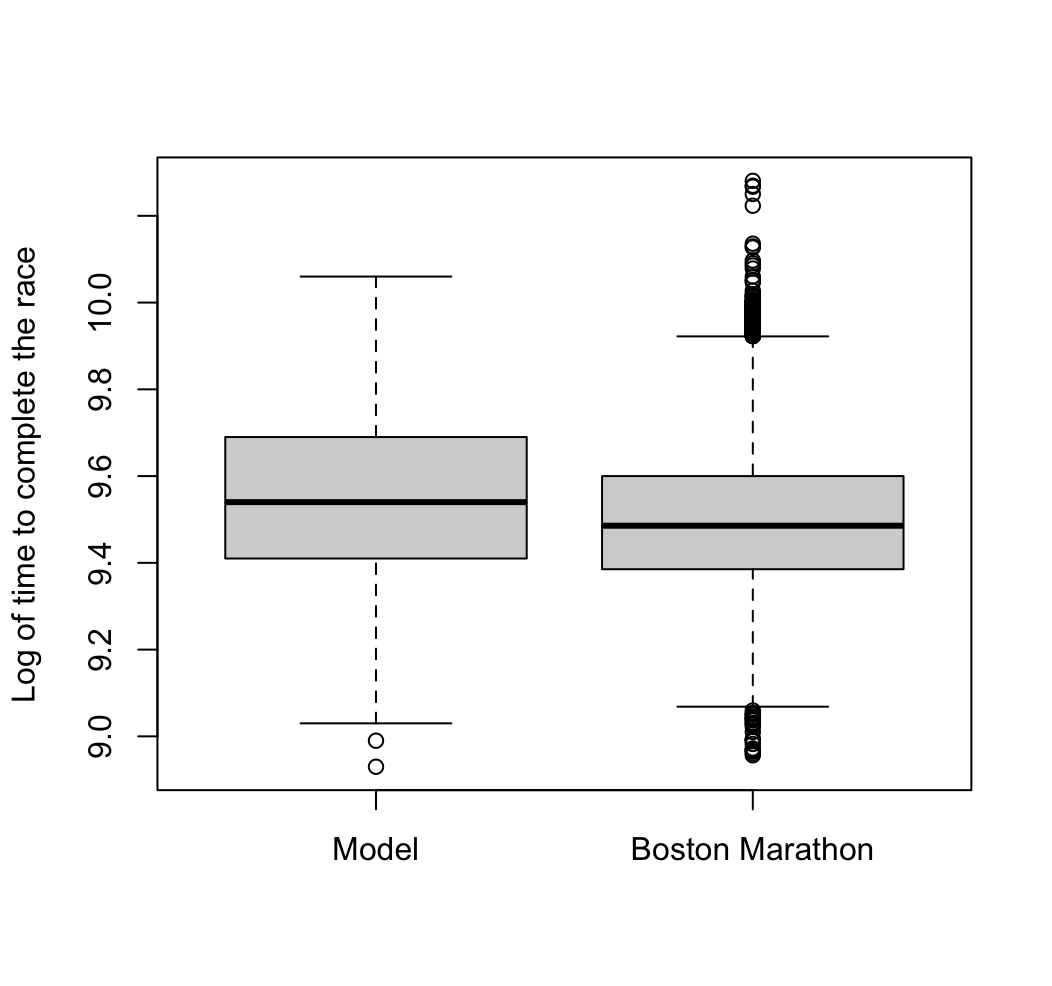
\includegraphics[width=\linewidth]{figs/blackbox_plot.png}}
        \caption{Box plots for the real dataset and the simulated results.}
        \label{fig:blackbox_plot}
    \end{figure}

    \item \textbf{Statistical Validation}
    First we ensure that the replications we have are enough to calculate the effects of the factors with 95\% confidence. By comparing the obtained confidence intervals with the desired ones in tables \ref{tab:rep_significance} and \ref{tab:rep_significance_2} we confirm that 16 repetitions is enough for every experiment. Furthermore we performed an ANOVA test on the log of the resulting race times for all 2000 entities of one run of the simulation per each scenario to see if the difference between them were statistically significant, available in table \ref{tab:anova_results}. The results of the ANOVA confirm that there are differences in the groups of experiments for each variable with 95\% confidence. We also performed assumption tests for the ANOVA and all normality, independence of observations and homogeneity of variance hold.

    \begin{table}[]
    \caption{Results and half ranges for simulation runs}
    \begin{center}
    \begin{tabular}{|c|c|c|c|c|c|c|c|c|}
    \hline
    \textbf{Temperature} & - & + & - & + \\
    \hline
    \textbf{Humidity} & - & - & + & + \\
    \hline
    \textbf{Supplies} &+&+&+&+ \\
    \hline
    \textbf{Res. Mean} & 14588.87&15051.87&14489.60&14952.23 \\
    \hline
    \textbf{S2}& 6751.25&7171.83&5285.16&4787.46 \\
    \hline
    \textbf{Variance}&3667.11&3783.47&3640.00&3754.81\\
    \hline
    \textbf{h} &43.548&44.884&38.531&36.671\\
    \hline
    \textbf{Desired h}&729.44&752.59&724.48&747.61\\
    \hline
    \end{tabular}
    \label{tab:rep_significance}
    \end{center}
    \end{table}

    \begin{table}[]
    \caption{Results and half ranges for simulation runs}
    \begin{center}
    \begin{tabular}{|c|c|c|c|c|c|c|c|c|}
    \hline
    \textbf{Temperature} & - & + & - & + \\
    \hline
    \textbf{Humidity} & - & - & + & + \\
    \hline
    \textbf{Supplies} &+&+&+&+ \\
    \hline
    \textbf{Res. Mean} & 14588.87&15051.87&14489.60&14952.23 \\
    \hline
    \textbf{S2}& 6751.25&7171.83&5285.16&4787.46 \\
    \hline
    \textbf{Variance}&3667.11&3783.47&3640.00&3754.81\\
    \hline
    \textbf{h}&43.548&44.884&38.531&36.671\\
    \hline
    \textbf{Desired h}&729.44&752.59&724.48&747.61\\
    \hline
    \end{tabular}
    \label{tab:rep_significance_2}
    \end{center}
    \end{table}

    \begin{table}[]
    \caption{ANOVA results for times against variables}
    \begin{center}
    \begin{tabular}{|c|c|c|c|c|c|}
    \hline
    & \textbf{Df} & \textbf{Sum Sq. } & \textbf{Mean Sq.} & \textbf{F value} & \textbf{p value} \\
    \hline
    \textbf{Temperature} & 1 & 7.72 & 7.715 & 841.49 & \textless 2e-16 \\
    \hline
    \textbf{Humidity} & 1 & 0.53 & 0.530 & 841.49  & 3.05e-14\\
    \hline
    \textbf{Supplies} & 1 & 26.45 & 26.448 & 57.81 & \textless 2e-16\\
    \hline
    \textbf{Residuals} & 15996 & 146.66 & 0.009 & & \\
    \hline
    \end{tabular}
    \label{tab:anova_results}
    \end{center}
    \end{table}

\end{enumerate}

\section{Results/Conclusions}
% NOT CONVINCED: The temperature effect may not be the most correctly used attribute of the enviorment. The effect of heat is based frm a range between 5 and 24.5 degrees, which is not a very wide range. The wind speed analysis does not seem to explain wind direction. Maybe its usually the same direction in this place.

By analysing the results of the simulation we can identify the most important factors in minimizing mean time to completion for the race. As illustrated in table \ref{tab:results}, these are mainly the availability of supplies followed by temperature (which should be minimized) and humidity (which should be maximized). The effect of interactions is comparatively very small but we can see that even though both supplies and humidity on their own reduce the race time, together they have an interaction that causes it to increase. This can likely be explained by lower times causing runners to bunch up, overcrowding resupply points.

\begin{table}[htbp]
\caption{Effects of factors on mean time to finish}
\begin{center}
\begin{tabular}{|c|c|c|c|c|c|c|c|c|}
\hline
\textbf{Temperature} & 462.680\\
\hline
\textbf{Humidity} & -99.483\\
\hline
\textbf{Supplies} & -686.567\\
\hline
\textbf{Temperature and Humidity} & 1.504\\
\hline
\textbf{Temperature and Supplies}& 0.133\\
\hline
\textbf{Humidity and Supplies}&0.023\\
\hline
\textbf{All}&-1.691\\
\hline
\end{tabular}
\label{tab:results}
\end{center}
\end{table}

Additionally we analyse the results from queue information from the simulation. We can see that even in the worst case we can by the time runners reached the end of the race they were spread out enough to not cause overcrowding of any station, while in the beginning of the race only about 5\% of runners were able to access them without queueing. This suggests that a more important factor to consider rather than global resource availability is how to distribute them along the race in ways that can be accessed by large crowds near the beginning.

\begin{table}[htbp]
\caption{Queue utilization for one simulation run (high temp. low hum. low sup.)}
\begin{center}
\begin{tabular}{|c|c|c|c|c|}
\hline
\textbf{Sup. point}&\textbf{Max. cont.}&\textbf{Avg. cont.}&\textbf{Zero ent.}&\textbf{Pct. zero}\\
\hline
1&858&58.79&96&4.80\\
\hline
2&27&0.36&1259&62.95\\
\hline
3&19&0.14&1574&78.70\\
\hline
4&10&0.02&1886&94.30\\
\hline
5&10&0.01&1937&96.85\\
\hline
6&5&0.00&1960&98.00\\
\hline
7&3&0.00&1990&99.50\\
\hline
8&1&0.00&1999&99.95\\
\hline
9&0&0.00&2000&100.00\\
\hline
10&0&0.00&2000&100.00\\
\hline
\end{tabular}
\label{tab:queue_results}
\end{center}
\end{table}

\subsection{Further work}

While we can use these results to make some decisions about the organization of the event the model provided is still fairly simple and limited. An avenue that remains unexplored is a more complete simulation of resupply points, their distribution along the race, supplying different resources at different times, etc. This model provides a basic overview of the effects of bottlenecks in the development of the race but isn't flexible enough to test different scenarios and provide answers that help organize a better and safer competition in this regard.

\newpage
\onecolumn
\section{Annex}

\begin{table}[h]
\caption{Effects of factors on mean time to finish}
\begin{center}
\begin{tabular}{|c|c|c|c|c|c|c|c|c|}
\hline
\textbf{Temp}&\textbf{Hum}&\textbf{Sup}&\textbf{Mean}&&&&\textbf{Effect}&\textbf{Meaning} \\
\hline
-&-&-&15277.28625&31013.925&61828.838125&120911.40875&15113.92609375&Mean \\
+&-&-&15736.63875&30814.913125&59082.570625&1850.72125&462.6803125&Temp \\
-&+&-&15174.585&29640.745625&925.095625&-397.9325&-99.483125&Humidity \\
+&+&-&15640.328125&29441.825&925.625625&6.0175&1.504375&Temp + Hum \\
-&-&+&14588.873125&459.3525&-199.011875&-2746.2675&-686.566875&Supplies \\
+&-&+&15051.8725&465.743125&-198.920625&0.53&0.1325&Temp + Sup \\ 
-&+&+&14489.599375&462.999375&6.390625&0.09125&0.0228125&Hum + Sup \\
+&+&+&14952.225625&462.62625&-0.373125&-6.76375&-1.6909375&All \\
\hline
\end{tabular}
\label{tab:rep_significance_2}
\end{center}
\end{table}

GPSS Simulation code:
\begin{verbatim}
SIMULATE 16

LEVEL FUNCTION RN1,R
0 82
1 4923
2 4938
GENE FUNCTION RN1,R
0 9360
1 639
GENH FUNCTION RN1,R
0 7030
1 2970
GENN FUNCTION RN1,R
0 3873
1 6126
RMEAN FUNCTION P$LEVEL,D
0 9.128
1 9.381
2 9.627
RSTD FUNCTION P$LEVEL,D
0 0.26298
1 0.30842
2 0.36145
HUM FUNCTION P$HUM,D
0 0
1 0
2 -103.8
3 -104.4
4 -126.6
5 -71.4
TEMP FUNCTION P$TEMP,D
0 0
1 0
2 71.4
3 82.8
4 463.8
5 466.8
LET X$STAGES=10
! Humidity value
INPUT X$HUM
LET X$SUPPL=20
! Temperature value
INPUT X$TEMP
1 CAPACITY X$SUPPL
2 CAPACITY X$SUPPL
3 CAPACITY X$SUPPL
4 CAPACITY X$SUPPL
5 CAPACITY X$SUPPL
6 CAPACITY X$SUPPL
7 CAPACITY X$SUPPL
8 CAPACITY X$SUPPL
9 CAPACITY X$SUPPL
10 CAPACITY X$SUPPL
RACE CAPACITY
Times TABLE P$TIME,0,1,1
TimLog TABLE P$TLOG,0,1,1
GENE VALUEOF FN$GENE*FN$EQ0(P$LEVEL)
GENH VALUEOF FN$GENH*FN$EQ0(P$LEVEL-1)
GENN VALUEOF FN$GENN*FN$EQ0(P$LEVEL-2)
GENDER VALUEOF V$GENE+V$GENH+V$GENN
TEMP VALUEOF X$TEMP*2+P$GENDER
HUM VALUEOF X$HUM*2+P$GENDER
RUN VALUEOF (FN$EXP(FN$SNORM*P$STD+P$MEAN)+FN$TEMP+FN$HUM)/X$STAGES
	GENERATE 0,,0,2000,2
* INITIALIZE  RUNNERS
	LET P$STAGE=1
	LET P$LEVEL=FN$LEVEL
	LET P$GENDER=V$GENDER
	LET P$TEMP=V$TEMP
	LET P$HUM=V$HUM
	LET P$MEAN=FN$RMEAN
	LET P$STD=FN$RSTD
* RACE SIMULATION
RACE_START	ENTER RACE
STAGE_START	ADVANCE V$RUN
	ARRIVE P$STAGE
	ENTER P$STAGE
	DEPART P$STAGE
	ADVANCE 30,20
	LEAVE P$STAGE
	LET+ P$STAGE,1
	IF P$STAGE<=X$STAGES,STAGE_START
	LEAVE RACE
	LET P$TIME=CL
	LET P$TLOG=FN$LOG(P$TIME)
	TABULATE Times
	TERMINATE 
* RACE CONTROL

	GENERATE ,,,1,0
	WAITIF RACE=NE
	TERMINATE 1

START 1
END

\end{verbatim}


\begin{thebibliography}{00}
% \bibitem{b1} G. Eason, B. Noble, and I. N. Sneddon, ``On certain integrals of Lipschitz-Hankel type involving products of Bessel functions,'' Phil. Trans. Roy. Soc. London, vol. A247, pp. 529--551, April 1955.
% \bibitem{b2} J. Clerk Maxwell, A Treatise on Electricity and Magnetism, 3rd ed., vol. 2. Oxford: Clarendon, 1892, pp.68--73.
% \bibitem{b3} I. S. Jacobs and C. P. Bean, ``Fine particles, thin films and exchange anisotropy,'' in Magnetism, vol. III, G. T. Rado and H. Suhl, Eds. New York: Academic, 1963, pp. 271--350.
% \bibitem{b4} K. Elissa, ``Title of paper if known,'' unpublished.
% \bibitem{b5} R. Nicole, ``Title of paper with only first word capitalized,'' J. Name Stand. Abbrev., in press.
% \bibitem{b6} Y. Yorozu, M. Hirano, K. Oka, and Y. Tagawa, ``Electron spectroscopy studies on magneto-optical media and plastic substrate interface,'' IEEE Transl. J. Magn. Japan, vol. 2, pp. 740--741, August 1987 [Digests 9th Annual Conf. Magnetics Japan, p. 301, 1982].
% \bibitem{b7} M. Young, The Technical Writer's Handbook. Mill Valley, CA: University Science, 1989.
\bibitem{b8} B. Knechtle, C. McGrath, O. Goncerz, E. Villiger, P. T. Nikolaidis, T. Marcin, and C. V. Sousa, ``The Role of Environmental Conditions on Master Marathon Running Performance in 1,280,557 Finishers the ‘New York City Marathon’ From 1970 to 2019,'' Frontiers in Physiology, vol. 12, 2021. [Online]. Available: https://www.frontiersin.org/journals/physiology/articles/10.3389/fphys.2021.665761. DOI: 10.3389/fphys.2021.665761. ISSN: 1664-042X.

\bibitem{math} Fonseca i Casas, P. A Continuous Process for Validation, Verification, and Accreditation of Simulation Models. Mathematics 2023, 11, 845. https://doi.org/10.3390/math11040845

\end{thebibliography}
\vspace{12pt}

\end{document}
